% This is the "preamble" of the document. This is where the format options get set.
% Pro-tip: things following the % mark will not be compiled by LaTeX. I'll be using them extensively to explain things as we go.
% Note: not to scare you off of LaTeX, but it's normal to have problems. And ya girl has been having some. I've included the copyright info at the bottom of the document from the guy who wrote this package, because his documentation doesn't entirely match how it's actually used. So this is a combination of his working preamble along with my added commentary or explanation.
%%
\documentclass[stu,12pt,floatsintext]{apa7}

\usepackage{booktabs}
\usepackage{tabularx}
\usepackage{lscape}
\usepackage{caption}
\captionsetup[table]{justification=centering}
\usepackage{adjustbox}
\usepackage[american]{babel}
\usepackage{authblk}
\usepackage{graphicx} % Required for including images
\usepackage{csquotes} % One of the things you learn about LaTeX is at some level, it's like magic. The references weren't printing as they should without this line, and the guy who wrote the package included it, so here it is. Because LaTeX reasons.
\usepackage[style=apa,sortcites=true,sorting=nyt,backend=biber]{biblatex}
% biblatex: loads the package that will handle the bibliographic info. Other option is natbib, which allows for more customization
% - style=apa: sets the reference format to use apa (albeit the 6th edition)
\DeclareLanguageMapping{american}{american-apa} % Gotta make sure we're patriotic up in here. Seriously, though, there can be local variants to how citations are handled, this sets it to the American idiosyncrasies
\addbibresource{references.bib} % This is the companion file to the main one you're writing. It contains all of the bibliographic info for your references. It's a little bit of a pain to get used to, but once you do, it's the best. Especially if you recycle references between papers. You only have to get the pieces in the holes once.`

\usepackage{comment}
\usepackage{siunitx}
\sisetup{round-mode=places,round-precision=2}
\usepackage[T1]{fontenc}
\usepackage{mathptmx} % This is the Times New Roman font, which was the norm back in my day. If you'd like to use a different font, the options are laid out here: https://www.overleaf.com/learn/latex/Font_typefaces
% Alternately, you can comment out or delete these two commands and just use the Overleaf default font. So many choices!


% Title page stuff
\title{Predicting a Successful Climb of Mount Everest} % The big, long version of the title for the title page
\shorttitle{What Defines a Successful Climb of Mount Everest} % The short title for the header
\authorsnames{Jacob Tassos, Mostafa Zamani Turk, Marston S. Ward}
\duedate{June 23, 2025}
% \date{January 17, 2024} The student version doesn't use the \date command, for whatever reason
\affiliation{University of San Diego}
\course{MS-AAI 500-01} % LaTeX gets annoyed (i.e., throws a grumble-error) if this is blank, so I put something here. However, if your instructor will mark you off for this being on the title page, you can leave this entry blank (delete the PSY 4321, but leave the command), and just make peace with the error that will happen. It won't break the document.
\professor{Professor Leonid Shpaner M.S.}  % Same situation as for the course info. Some instructors want this, some absolutely don't and will take off points. So do what you gotta.

\abstract{Abstract to be written later}

%\keywords{APA style, demonstration} % If you need to have keywords for your paper, delete the % at the start of this line

\begin{document}
\maketitle % This tells LaTeX to make the title page

% \section{Introduction} This command is commented out, because I was taught it was redundant to have the paper's title and introduction together. If your instructor wants it to say "Introduction", delete the % at the start

\section{Introduction}
Mount Everest is the highest land surface point on the planet, when this height is defined as height above mean sea level. At \si{8,848~\km} (\si{29,031.7~feet}), it towers above it's closest rival by more than \si{200~\km} (See list of highest mountains on Earth: \url{https://en.wikipedia.org/wiki/List_of_highest_mountains_on_Earth}). While there are more than 100 peaks on the planet with peaks above \si{7~\km}, none captures the human imagination as Everest. Humans cannot live at such high elevations far above the tree line, where the air is rarefied and every function of the human body is challenged (\cite{gooshow2018}).

Despite the extreme environment of peaks about 7,000 km, the human desire to overcome a challenge even at extremely personal risk remains alive and well. Mountains are not the only extreme environment on the planet that humans have tried to reach. The deepest parts of the oceans are also areas we have successfully traversed, however, the costs of specialized equipment and availability of aid in achieving the goal of reaching these extreme environment has made Everest an attractive place because it became attainable and relatively inexpensive.

For centuries now, climbing the worlds highest mountains has been enabled and facilitated by modern technology and, in the case of Everest, Nepal tourist industry built around climbing the mountain. These two factors have made one of the world's deadliest mountains accessible to even more adventurers, and many would say, amateurs. In the early days of climbing, teams climb to be the first to reach the highest peak. Now, anyone with enough resources can travel to the peaks, especially Everest, and attempt to summit. But far from all who attempt the climb make it, or even make it back in one piece - if they make it back at all.

Everest and K2 (second peak in Karakoram) have over the years competed for the title: deadliest mountain. Many lives have been lost due a range of factors ranging from physiology, mindset, preparedness, ego, stupidity and natural disasters such as avalanches and inclement weather. Many studies and documentaries have been done on mountain climbers and their plight to summit and return - alive. But sadly, the history of climbing is replete with tragedies. In the light of this some articles have tried to analyze and suggest ways to improve your chances of a successful summit. In this paper we define that success as one way where the climber summits but not necessarily returns. For example, \textcite{hueymountaineering2001} analyzed a research program that attempted to predict (similar to this paper) what factors influence the success ascent or death rates. In this project, we do not try to predict death rates as not all failures to summit is due to accidents or deaths. However, the paper drew no conclusions on the matter. \textcite{szymczakcomparison2021} examined the weather climber experienced on Everest and K2 in both the climbing season (July) and mid winter season. They study found that more extreme weather in both seasons than on K2, which is \si{8^{\circ}} latitude farther north.


\section{Dataset}
The chosen dataset, expeditions.csv, is a file with 10,511 rows and 57 columns. Each row represents an expedition that took place between 1905 and 2020, and each column corresponds to a measured feature of that expedition. Among these features is the variable "mbrs\_summited," which indicates the total number of members that reached the peak. This variable will be used to define the terms of success. After converting it to a binary variable, it will show whether any member of the expedition made it to the summit or not. Thus, an expedition is successful if at least one member reaches the peak. It is worth noting that expeditions vary in size, with a differing number of members participating in each. Since only the ascent will be necessary for the definition of success, not every feature will be used. Some of the useful features include the following: peak name, year, season, leader(s), the first through fourth routes taken, a commercial or standard route, intermediate points before the summit, total number of days, total number of members, if oxygen was used during ascent, agency name, and a list of members.


\section{Exploratory Data Analysis}
Number of expeditions in the raw file are 10,511. After initial feature selection and removing rows 
with NaNs, that number drops to 4,346.  The statistical description of the selected variables chosen show the following characteristics:
\begin{itemize}
    \item year: Expeditions span 1972–2020 (mean 2008.5, median 2009), concentrated in recent decades.
    \item season: Encoded 1–4, expeditions occur across all seasons.
    \item rte\_1\_name: Wide variety of routes (1–459), median route code 28, high variability.
    \item is\_disputed and is\_claim: Very rare (means near zero), most expeditions are undisputed and uncontested.
    \item is\_commercial\_rte \& is\_standard\_rte: About 57\% use commercial or standard routes (median 1).
    \item approach: Diverse approaches (range 1–2041), median 652, high variability.
    \item total\_days: Most expeditions last about 21 days (median), but range from 0 to 280 days.
    \item max\_elev\_reached: Typical maximum elevation is 7,400 m (median), with a range up to 8,850 m.
    \item mbrs\_deaths: Deaths are rare (median 0, max 10).
    \item is\_o2\_climbing: 30\% used supplemental oxygen (median 0, 75th percentile 1).
    \item agency: Many organizing agencies (codes 1–603), median code 66.
    \item members: Team sizes are large on average (mean 2,121, median 2,111), with wide variation.
    \item exp\_result: 1 (“success”) is the most common outcome (2,458 out of 4,346; approximately 57\%), 
    0 otherwise.

The dataset covers a broad range of expeditions, mostly in the 21st century, with most teams using standard/commercial routes and achieving high elevations. Success is the most frequent result, and fatalities or disputes are rare.
\end{itemize}


\begin{table}[ht]
\centering
\caption{The variable IDs are mapped as follows:
PN=peak\_name, Y=year, S=season, L=leader(s), R1=rte\_1\_name, CR=is\_commercial\_rte, SR=is\_standard\_rte, AP=approach, TD=total\_days, ME=max\_elev\_reached, TM=total\_mbrs, O2=is\_o2\_climbing, AG=agency, MB=members}
\begin{tabular}{lrrrr}
\toprule
\textbf{Variable} & \textbf{Acc.} & \textbf{PN Acc.} & \textbf{PN and O2 Acc.} & \textbf{PN, O2, and TD Acc.} \\
\midrule
PN & 0.69133 & -       & -       & -       \\
Y  & 0.68376 & 0.70143 & 0.73675 & 0.74012 \\
S  & 0.68545 & 0.70059 & 0.73591 & 0.74180 \\
L  & 0.68881 & 0.69386 & 0.72918 & 0.73759 \\
R1 & 0.69807 & 0.71993 & 0.73507 & 0.74348 \\
R2 & 0.68797 & 0.69134 & 0.73171 & 0.74937 \\
R3 & 0.68797 & 0.69134 & 0.73003 & 0.74853 \\
R4 & 0.68797 & 0.69134 & 0.73003 & 0.74853 \\
CR & 0.68797 & 0.69470 & 0.73423 & 0.74180 \\
SR & 0.68797 & 0.70395 & 0.73760 & 0.74516 \\
AP & 0.68629 & 0.69050 & 0.74601 & 0.74601 \\
TD & 0.68713 & 0.69134 & 0.74853 & -       \\
ME & 0.98738 & 0.98738 & 0.98654 & 0.98570 \\
TM & 0.68797 & 0.68545 & 0.73759 & 0.74432 \\
O2 & 0.68797 & 0.73003 & -       & -       \\
AG & 0.68293 & 0.70059 & 0.74516 & 0.75105 \\
MB & 0.69554 & 0.70059 & 0.73591 & 0.74601 \\
\bottomrule
\end{tabular}
\label{tab:summary_stats}
\end{table}


\begin{landscape}
\setlength{\tabcolsep}{4pt} % reduce horizontal padding between columns (default ~6pt)
\renewcommand{\arraystretch}{1.1} % adjust row height for readability
\begin{table}[htbp]
\centering
\caption{Summary statistics for expedition variables. The variable IDS are mapped as follows:
Y=year, S=season, R1=rte\_1\_name, D=is\_disputed, C=is\_claim, CR=is\_commercial\_rte, SR=is\_standard\_rte, 
AP=approach, TD=total\_days, ME=max\_elev\_reached, MD=mbrs\_deaths=O2, is\_o2\_climbing, AG=agency, MB=members,
ER=exp\_result}
\label{tab:expedition_summary}
\begin{tabularx}{\linewidth}{l*{15}{>{\centering\arraybackslash}X}}
\toprule
 & Y & S & R1 & D & C & CR & SR & AP & TD & ME & MD & O2 & AG & MB & ER \\
\midrule
count & 4346 & 4346 & 4346 & 4346 & 4346 & 4346 & 4346 & 4346 & 4346 & 4346 & 4346 & 4346 & 4346 & 4346 & 4346 \\
mean & 2008.53 & 2.04 & 84.73 & 0.01 & 0.00 & 0.57 & 0.57 & 833.91 & 22.22 & 7345.27 & 0.05 & 0.30 & 120.68 & 2121.51 & 0.57 \\
std & 7.89 & 1.02 & 106.47 & 0.07 & 0.05 & 0.50 & 0.50 & 567.77 & 15.36 & 1376.33 & 0.34 & 0.46 & 134.22 & 1226.52 & 0.50 \\
min & 1972 & 1 & 1 & 0 & 0 & 0 & 0 & 1 & 0 & 0 & 0 & 0 & 1 & 1 & 0 \\
25\% & 2005 & 1 & 3 & 0 & 0 & 0 & 0 & 411.25 & 11 & 6700 & 0 & 0 & 29 & 1064.25 & 0 \\
50\% & 2009 & 3 & 28 & 0 & 0 & 1 & 1 & 652 & 21 & 7400 & 0 & 0 & 66 & 2111.5 & 1 \\
75\% & 2015 & 3 & 126.75 & 0 & 0 & 1 & 1 & 1271 & 32 & 8188 & 0 & 1 & 157 & 3181.75 & 1 \\
max & 2020 & 4 & 459 & 1 & 1 & 1 & 1 & 2041 & 280 & 8850 & 10 & 1 & 603 & 4258 & 1 \\
\bottomrule
\end{tabularx}
\end{table}
\end{landscape}


\begin{figure*}[h!]
    \centering
    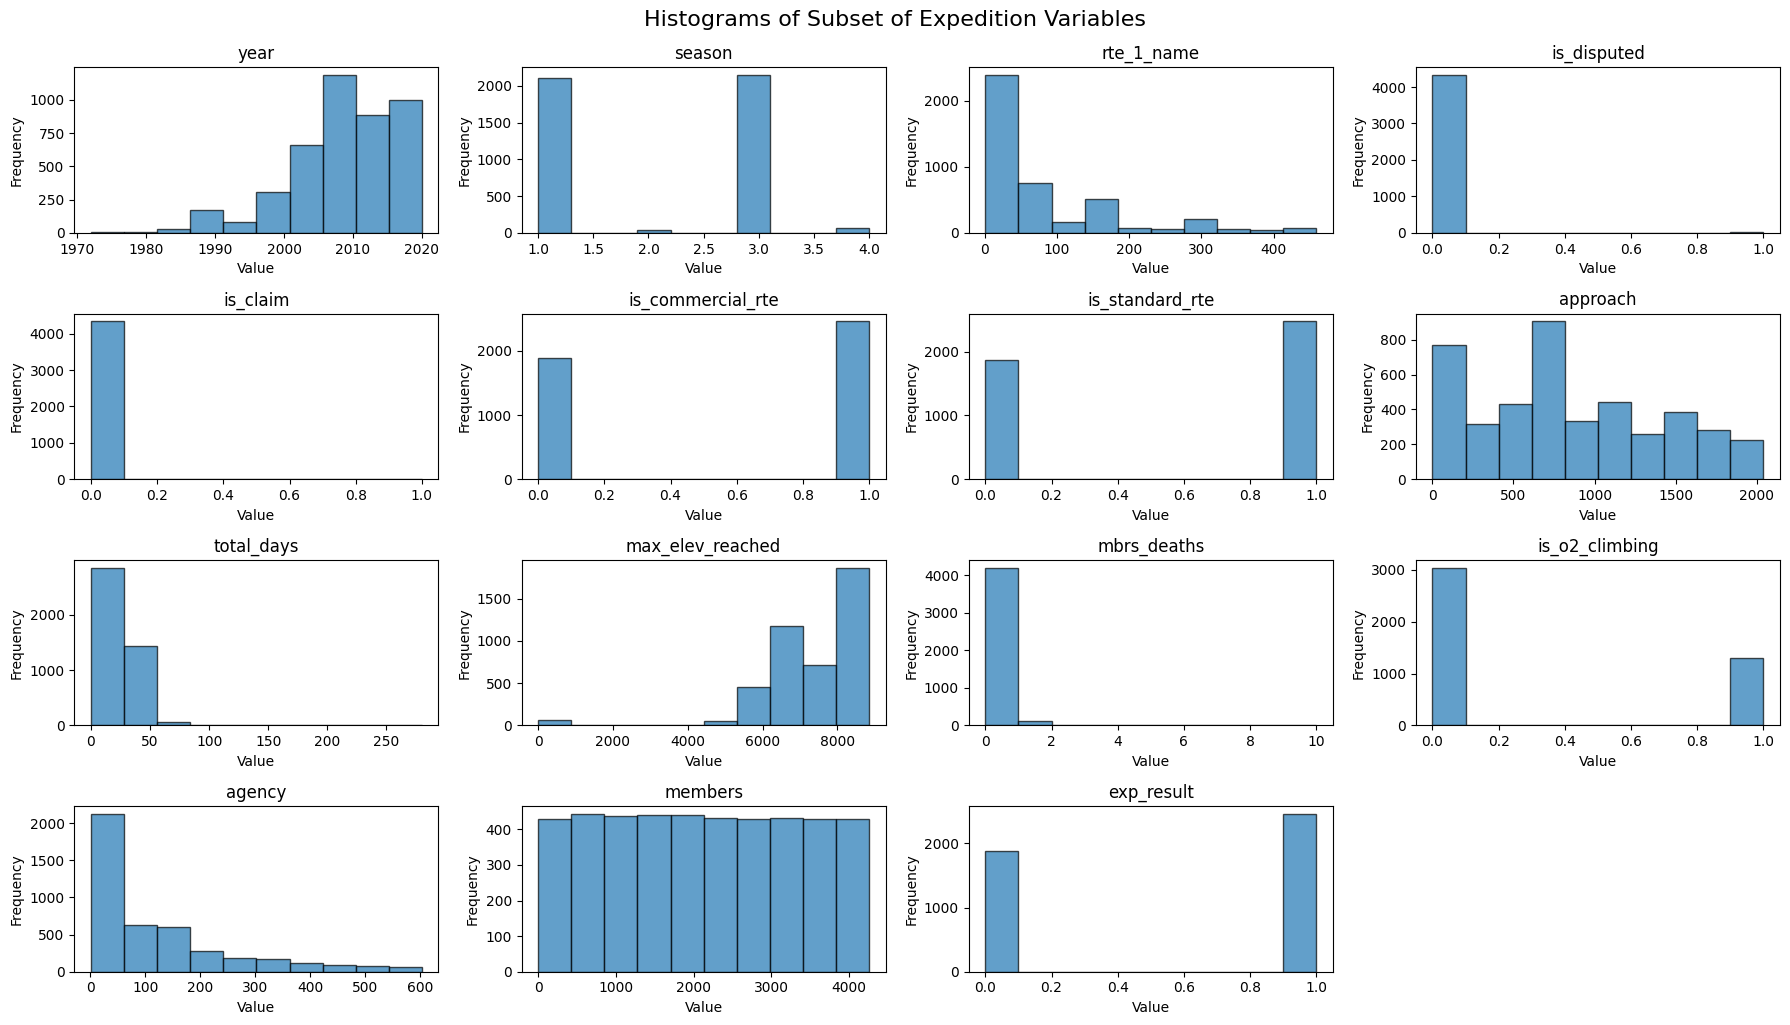
\includegraphics[width=1.0\textwidth]{eda.png} 
    \caption{Histogram plots of the input features.}
    \label{fig:eda}
\end{figure*}

\end{document}
